\documentclass{article}
\usepackage{iclr2026_conference,times}

\input{math_commands.tex}

\usepackage{amsmath}
\usepackage{amssymb}
\usepackage{mathtools}
\usepackage{booktabs}
\usepackage{graphicx}
\usepackage{float}
\usepackage{hyperref}
\usepackage{url}

\title{MatrixPolicy: Role-Aware Optimization for Rational Transformer Nonlinearities}

\author{Anonymous Authors}

\newcommand{\clip}{\operatorname{clip}}
\newcommand{\rms}{\operatorname{rms}}
\newcommand{\geom}{\operatorname{geomean}}
\newcommand{\relu}{\operatorname{ReLU}}
\newcommand{\smooth}{\operatorname{smoothstep}}
\newcommand{\RLB}{\mathrm{RLB}}
\newcommand{\diag}{\operatorname{diag}}

\begin{document}

\maketitle

\begin{abstract}
Transformer nonlinear sublayers contain an input matrix, a coordinatewise
nonlinearity, and an output matrix, but standard optimizers usually update the
two matrices without using their different functional roles.  We introduce a
global-rational Rational Latent Basis (RLB) sublayer that exposes normalized
group coordinates, trainable real-pole-free P5/Q4 responses, curve-gain proxies,
and a positive matrix-pair rescaling structure.  We then introduce MatrixPolicy,
a role-aware optimizer that acts only on the RLB input and output matrices while
leaving rational coefficients and all other Transformer parameters on AdamW.
MatrixPolicy combines centered group-gradient redistribution, an early
matrix-direction branch, and bounded matrix-pair balancing.  The central benefit
is optimization speed through useful loss levels, not only endpoint loss after a
long fixed budget.  On five 12-layer, width-768 language-model pretraining
corpora, MatrixPolicy reaches E2 validation-loss targets with 9.8--37.7M fewer
tokens than the fastest reachable non-MatrixPolicy comparator and 51.9--69.9M
fewer tokens than SiLU+AdamW; using measured throughput, these token savings also
translate into lower estimated training time in all five E2 datasets.  After the
full 300M-token budget, where strong baselines have more time to approach their
own saturation levels, MatrixPolicy still preserves lower endpoint validation
loss across all five datasets.
\end{abstract}

\section{Introduction}
\label{sec:introduction}

Transformer nonlinear sublayers are usually described by their scalar activation:
GELU, SiLU, SwiGLU, or a related gated variant
\citep{hendrycks2016gelu,ramachandran2017swish,shazeer2020glu}.  That shorthand
hides a larger optimization object.  A sublayer first chooses coordinates through
an input matrix, applies a nonlinear response in those coordinates, and then
recombines the resulting features through an output matrix.  The two matrices do
not play the same role, yet AdamW, Lion, Muon, and other general optimizers
usually see them as ordinary tensors with no knowledge of which side of the
nonlinearity they occupy.

This paper studies whether the nonlinear sublayer can expose enough structure for
the optimizer to use.  The key idea is to make the activation an interface, not
only a pointwise function.  If the sublayer provides normalized groups, a
trainable rational response in each group, observable derivative and curve-response
scales, and a controlled positive rescaling relation between the adjacent
matrices, then the optimizer can assign different update behavior to the input
and output roles without changing the rest of the Transformer.

We instantiate this idea with Rational Latent Basis (RLB).  RLB projects the
residual stream into grouped latent coordinates, RMS-normalizes each group,
applies one trainable real-pole-free P5/Q4 response per group, and projects back to
the model width.  The main variant used in this paper has no active local atoms:
there are no trainable atom centers and no atom coefficient parameters.  This
choice keeps the nonlinear response simple enough to audit while preserving the
signals that MatrixPolicy uses.

MatrixPolicy is the optimizer coupled to this sublayer.  It is not a generic
optimizer for every Transformer tensor.  It acts only on the two RLB matrices,
using batch-estimated rational gain proxies, relative gradient scales, and the matrix
pair ratio to redistribute group updates, select a transient early matrix-direction
branch, and keep the input/output representatives balanced.  Rational
coefficients, attention weights, embeddings, and all other non-RLB-matrix
parameters remain on AdamW.

We evaluate the method on a fixed 12-layer, width-768 causal Transformer across
DCLM, FineWeb-Edu, FineWeb, Dolma-sample, and C4.  The longer 300M-token regime
is deliberately a saturation test: strong activation/optimizer choices continue
to improve for many more steps, so endpoint gaps naturally compress compared with
the 100M-token regime.  We therefore make the main empirical question sharper:
how quickly does a method move through useful validation-loss levels, and does it
still keep an endpoint advantage once the full budget is spent?  MatrixPolicy
answers both.  It reaches representative E2 targets with fewer tokens and lower
estimated training time than the fastest reachable non-MatrixPolicy comparator
and than SiLU+AdamW, while still ending with the lowest aggregate validation loss
on all five E2 datasets.

The contributions are:
\begin{itemize}
    \item a global-rational RLB sublayer that exposes matrix roles, curve-gain
    summaries, and a positive matrix-pair rescaling structure without local atom
    parameters;
    \item MatrixPolicy, a role-aware optimizer for the RLB input and output
    matrices that leaves rational coefficients and all non-RLB-matrix parameters
    on AdamW;
    \item a matched empirical package showing faster E2 target arrival in both
    tokens and estimated training time, plus persistent fixed-budget endpoint
    gains over SiLU and global-rational RLB controls across five corpora.
\end{itemize}

\section{Method}
\label{sec:method}

RLB and MatrixPolicy are designed as an activation--optimizer pair.  RLB defines
the nonlinear sublayer and exposes the statistics; MatrixPolicy consumes those
statistics to update only the adjacent input and output matrices.  Throughout the
method we use
\begin{align}
    \clip(x,a,b)&=\min\{\max\{x,a\},b\}, \\
    \smooth(a,b,x)&=3\omega^2-2\omega^3,
    \qquad
    \omega=\clip\left(\frac{x-a}{b-a},0,1\right).
\end{align}

\begin{figure}[H]
\centering
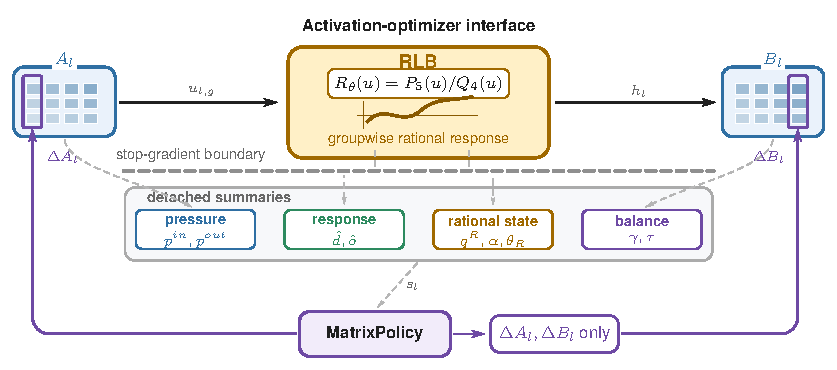
\includegraphics[width=0.97\linewidth]{figures/matrixpolicy_overview.pdf}
\caption{RLB exposes the input matrix, normalized rational groups, and output
matrix as separate optimizer-visible objects.  MatrixPolicy uses relative
gradient scales, batch-estimated derivative/response gains, and the matrix-pair
ratio to update only the RLB input/output matrices.}
\label{fig:matrixpolicy-overview}
\end{figure}

\subsection{Rational Latent Basis Sublayer}
\label{sec:method-rlb}

For Transformer layer $l\in\{1,\ldots,L\}$, let
$x_l\in\mathbb{R}^{d}$ denote the input to the nonlinear sublayer.  RLB first
projects this input to a latent width $H=Gm$ and partitions the latent vector
into $G$ groups of width $m$:
\begin{align}
    z_l=A_lx_l,
    \qquad
    z_l=\operatorname{concat}_{g=1}^{G}z_{l,g},
    \qquad
    z_{l,g}\in\mathbb{R}^{m},
    \label{eq:rlb-projection}
\end{align}
where $A_l\in\mathbb{R}^{H\times d}$ is the input-domain matrix.  Each group is
normalized by its root-mean-square radius,
\begin{align}
    r_{l,g}
    =
    \sqrt{m^{-1}\lVert z_{l,g}\rVert_2^2+\epsilon_{\rm rms}},
    \qquad
    u_{l,g}=z_{l,g}/r_{l,g},
    \label{eq:rlb-normalization}
\end{align}
with numerical floor $\epsilon_{\rm rms}>0$.  A scalar response is applied
coordinatewise in the normalized coordinates and then multiplied by the same
radius:
\begin{align}
    h_{l,g}=r_{l,g}R_{l,g}(u_{l,g}),
    \qquad
    h_l=\operatorname{concat}_{g=1}^{G}h_{l,g},
    \qquad
    y_l=B_lh_l,
    \label{eq:rlb-output}
\end{align}
where $B_l\in\mathbb{R}^{d\times H}$ is the output-recombination matrix.

The curve $R_{l,g}$ is a trainable real-pole-free piecewise-rational P5/Q4 response,
\begin{align}
    R_{l,g}(u)=\frac{P_{l,g}(u)}{Q_{l,g}(u)},
    \qquad
    P_{l,g}(u)=\sum_{i=0}^{5}a_{l,g,i}u^i,
    \label{eq:global-rational-p}
\end{align}
with denominator
\begin{align}
    Q_{l,g}(u)
    =
    1+|b_{l,g,1}|\,|u|+|b_{l,g,2}|\,u^2
     +|b_{l,g,3}|\,|u|^3+|b_{l,g,4}|\,u^4 .
    \label{eq:global-rational-q}
\end{align}
The absolute-value terms make the response piecewise rational rather than a
single algebraic rational function of $u$, but they guarantee $Q_{l,g}(u)\ge 1$
on the real line.  Numerator and denominator coefficients are initialized by
fitting SiLU on $[-5,5]$ and are trained thereafter.  The implementation uses the
same interval for probe-grid gain summaries.  In the main variant there are no
active local Cauchy atoms, trainable atom centers, or atom coefficient parameters.

The normalization in \eqref{eq:rlb-normalization} gives the optimizer two views
of each group.  The normalized coordinate $u_{l,g}$ determines where the response
is evaluated, while the radius $r_{l,g}$ carries group scale back to the residual
stream.  For fixed curves $R_l=\{R_{l,g}\}_{g=1}^{G}$, define the RLB block map
\begin{align}
    f_l(x;A_l,B_l,R_l)
    =
    B_l\operatorname{concat}_{g=1}^{G} r_{l,g}R_{l,g}(u_{l,g}),
    \label{eq:rlb-block-map}
\end{align}
where $z_l=A_lx$, $z_{l,g}$, $r_{l,g}$, and $u_{l,g}$ are computed by
\eqref{eq:rlb-projection}--\eqref{eq:rlb-normalization}.  In the idealized case
$\epsilon_{\rm rms}=0$ with nonzero group radii, this construction admits the
positive rescaling
\begin{align}
    f_l(x;A_l,B_l,R_l)
    =
    f_l(x;D_l(a)A_l,B_lD_l(a)^{-1},R_l),
    \label{eq:positive-rescale}
\end{align}
where $D_l(a)=\diag(a_1I_m,\ldots,a_GI_m)$ for
$a\in\mathbb{R}_{>0}^{G}$.  MatrixPolicy uses this relation only for small,
bounded balancing steps because the RMS floor makes the block-map identity approximate, and unchanged
optimizer state makes subsequent dynamics non-invariant in the implemented
system.

\subsection{Role-Aware Optimizer Statistics}
\label{sec:method-signals}

MatrixPolicy tracks role-specific relative gradient scales and curve-gain
summaries for each layer and group.  For any tensor $V$, define
\begin{align}
    \rms(V)=\sqrt{\operatorname{mean}(V^2)},
    \qquad
    \rms_{\epsilon}(V)=\max\{\rms(V),\epsilon\}.
    \label{eq:rms-definition}
\end{align}
The constants $\epsilon_p>0$ and $\epsilon_g>0$ denote fixed numerical floors
for pressure and gain summaries.  Let $A_{l,g}\in\mathbb{R}^{m\times d}$ be the row block of $A_l$, and let
$B_{l,g}\in\mathbb{R}^{d\times m}$ be the column block of $B_l$.  The relative
matrix-gradient scales are
\begin{align}
    p^{\rm in}_{l,g}
    =
    \frac{\rms_{\epsilon_p}(\nabla A_{l,g})}
    {\rms_{\epsilon_p}(A_{l,g})},
    \qquad
    p^{\rm out}_{l,g}
    =
    \frac{\rms_{\epsilon_p}(\nabla B_{l,g})}
    {\rms_{\epsilon_p}(B_{l,g})} .
    \label{eq:matrix-pressure}
\end{align}
The coefficient-gradient energy scale for the global response is
\begin{align}
    p^{R}_{l,g}
    =
    \left[
    \frac{1}{2}
    \left(
    \operatorname{mean}((\nabla a_{l,g,\cdot})^2)
    +
    \operatorname{mean}((\nabla b_{l,g,\cdot})^2)
    \right)
    +\epsilon_p^2
    \right]^{1/2}.
    \label{eq:rational-activity-raw}
\end{align}
MatrixPolicy maintains exponential moving averages
$q^{\rm in}_{l,g}$, $q^{\rm out}_{l,g}$, and $q^R_{l,g}$ of these quantities with
decay $0.95$, and forms
\begin{align}
    \pi_{l,g}
    =
    \log q^{\rm in}_{l,g}-\log q^{\rm out}_{l,g},
    \qquad
    \alpha_{l,g}
    =
    \log q^{R}_{l,g}
    -\frac{1}{2}\left(\log q^{\rm in}_{l,g}+\log q^{\rm out}_{l,g}\right).
    \label{eq:pressure-activity}
\end{align}
Here $\pi_{l,g}$ compares the update scale of the two adjacent matrix roles.
The score $\alpha_{l,g}$ is a heuristic coefficient-activity statistic: because
$p^R_{l,g}$ is an average of numerator- and denominator-gradient energies rather
than a dimensionless matrix pressure, MatrixPolicy uses $\alpha_{l,g}$ only
inside bounded redistribution and gating rules.

The activation also provides batch-estimated curve gains.  From a recent sample
of normalized coordinates $u_{l,g}$ cached by the RLB forward path, MatrixPolicy
uses floored summaries
\begin{align}
    \hat d^{\rm live}_{l,g}
    =
    \max\{\rms(R'_{l,g}(u_{l,g})),\epsilon_g\},
    \qquad
    \hat o^{\rm live}_{l,g}
    =
    \max\{\rms(R_{l,g}(u_{l,g})),\epsilon_g\}.
    \label{eq:live-gains}
\end{align}
The derivative gain is a proxy for the input-domain role.  The output gain is a
curve-response proxy for the recombination role; it does not include the group
radius $r_{l,g}$ and therefore is not the full feature scale seen by $B_l$.
Both gains are deliberately cheap summaries rather than full block-Jacobian
preconditioners.

\subsection{MatrixPolicy Update Rule}
\label{sec:method-update}

Let $t$ be the optimizer step, $T$ the planned number of training steps, and
$\xi_t=t/T$.  A smooth gate
\begin{align}
    \phi_t=\smooth(0.02,0.30,\xi_t)
    \label{eq:group-phase}
\end{align}
turns on the group-gradient policy.  For positive group values $v_j$, write
$\geom_j v_j=\exp(G^{-1}\sum_{j=1}^{G}\log v_j)$.  The multiplier for group
$g$ and role $r\in\{\mathrm{in},\mathrm{out}\}$ is
\begin{align}
    c_{l,g,r}
    =
    c^{\rm gain}_{l,g,r}
    c^{\rm pressure}_{l,g,r}
    c^{\rm activity}_{l,g}.
    \label{eq:group-multiplier}
\end{align}
For the input role, the gain term uses $\hat d^{\rm live}_{l,g}$; for the output
role, it uses $\hat o^{\rm live}_{l,g}$:
\begin{align}
    c^{\rm gain}_{l,g,\mathrm{in}}
    =
    \left(\frac{\geom_j \hat d^{\rm live}_{l,j}}{\hat d^{\rm live}_{l,g}}\right)^{0.20\phi_t},
    \qquad
    c^{\rm gain}_{l,g,\mathrm{out}}
    =
    \left(\frac{\geom_j \hat o^{\rm live}_{l,j}}{\hat o^{\rm live}_{l,g}}\right)^{0.20\phi_t}.
    \label{eq:gain-policy}
\end{align}
With $\tilde{\pi}_{l,g}=\clip(\pi_{l,g},-1.50,1.50)$, the relative-gradient term
sets role-dependent group multipliers before the later role-wise recentering:
\begin{align}
    c^{\rm pressure}_{l,g,\mathrm{in}}
    =
    \exp(-0.10\phi_t\tilde{\pi}_{l,g}),
    \qquad
    c^{\rm pressure}_{l,g,\mathrm{out}}
    =
    \exp(+0.10\phi_t\tilde{\pi}_{l,g}).
    \label{eq:pressure-policy}
\end{align}
Coefficient-gradient activity downweights groups whose rational coefficients are
moving more strongly than the adjacent matrices before role-wise recentering:
\begin{align}
    c^{\rm activity}_{l,g}
    =
    \exp\left[
    -0.20\phi_t
    \relu\left(\frac{\alpha_{l,g}-0.05}{0.45}\right)
    \right].
    \label{eq:activity-policy}
\end{align}
The final multiplier is recentered and clipped,
\begin{align}
    c_{l,g,r}\leftarrow
    \frac{c_{l,g,r}}{\geom_j c_{l,j,r}},
    \qquad
    c_{l,g,r}\leftarrow\clip(c_{l,g,r},0.75,1.35),
    \label{eq:group-center-clip}
\end{align}
so the policy redistributes update scale across groups, separately for each
matrix role, without changing the role-wise mean log multiplier before
clipping.

The scaled matrix gradients are
\begin{align}
    \widetilde\nabla A_{l,g}=c_{l,g,\mathrm{in}}\nabla A_{l,g},
    \qquad
    \widetilde\nabla B_{l,g}=c_{l,g,\mathrm{out}}\nabla B_{l,g}.
    \label{eq:scaled-gradients}
\end{align}
After this scaling, the RLB matrices are updated by a role/depth AdamW branch and
a transient Muon branch.  Define $\delta_l=(l-1)/(L-1)$ for $L>1$ and
$\delta_l=1/2$ otherwise.  The role factors are
\begin{align}
    \rho_{\mathrm{in}}(l)
    =
    \clip(1-0.50(\delta_l-0.5),0.55,1.40),
    \qquad
    \rho_{\mathrm{out}}(l)
    =
    \clip(1+1.00(\delta_l-0.5),0.55,1.40),
    \label{eq:role-factors}
\end{align}
and the AdamW matrix multiplier for role $r$ is
\begin{align}
    s^{\rm Adam}_{l,r}
    =
    \clip\left(
    3.0\max\{0.10,1+1.20(\rho_r(l)-1)\},
    0.40,4.0
    \right).
    \label{eq:adam-role-scale}
\end{align}
The Muon branch is concentrated early in training and is reduced when relative
scale imbalance or coefficient-gradient scale is high.  Define
\begin{align}
    \Psi_{l,t}
    =
    \frac{1}{G}\sum_{g=1}^{G}
    \left|\clip(\pi_{l,g},-1.50,1.50)\right|,
    \qquad
    \Omega_{l,t}
    =
    \frac{1}{G}\sum_{g=1}^{G}
    \relu\left(\frac{\alpha_{l,g}-0.05}{0.45}\right),
    \label{eq:pressure-activity-aggregates}
\end{align}
\begin{align}
    \psi_{l,t}
    =
    \clip\left(\exp[-0.30\Psi_{l,t}-0.65\Omega_{l,t}],0.10,1.15\right).
    \label{eq:stat-penalty}
\end{align}
The branch fraction is
\begin{align}
    \mu_{l,r,t}
    =
    \clip\left(
    0.75\,
    \smooth(0.02,0.12,\xi_t)
    [1-\smooth(0.20,0.36,\xi_t)]
    \rho_r(l)\psi_{l,t},
    0,0.75
    \right).
    \label{eq:muon-fraction}
\end{align}
For $M_{l,\mathrm{in}}=A_l$ and $M_{l,\mathrm{out}}=B_l$, MatrixPolicy composes
an AdamW matrix step with the Muon branch:
\begin{equation}
\begin{gathered}
    \widetilde M_{l,r}^{\,t+1}
    =
    \operatorname{AdamW}_{\eta_t s^{\rm Adam}_{l,r}(1-\mu_{l,r,t})}
    (M_{l,r}^{t};\widetilde\nabla M_{l,r}^{t}),\\
    M_{l,r}^{t+1}
    =
    \operatorname{Muon}_{\eta_t\mu_{l,r,t}}
    (\widetilde M_{l,r}^{\,t+1};\widetilde\nabla M_{l,r}^{t}),
\end{gathered}
    \label{eq:matrix-branch-step}
\end{equation}
Equation~\eqref{eq:matrix-branch-step} is operational update notation: AdamW and Muon
carry their own optimizer states, weight-decay and momentum terms are handled by
those optimizers, and both substeps use the gradient from training step $t$.
Here $\eta_t$ is the base learning rate and $\operatorname{Muon}$ denotes the
\texttt{torch.optim.Muon} update on two-dimensional RLB matrix parameters:
momentum $0.95$, five Newton--Schulz orthogonalization steps, and the match-RMS
learning-rate adjustment of the Muon optimizer \citep{liu2025muon}.  When all
Muon fractions have decayed to zero, this branch is inactive.

The last operation is a bounded positive rescaling of the two matrix blocks
around each rational curve.  It is evaluated every five optimizer steps; on other
steps it is skipped.  Let $\mathcal{U}=\{u_k\}_{k=1}^{129}$ be a uniform probe
grid over $[-5,5]$, and define
$\rms_{\mathcal{U}}(\varphi)=\sqrt{|\mathcal{U}|^{-1}\sum_{u_k\in\mathcal{U}}\varphi(u_k)^2}$.
The probe gains are
\begin{align}
    \hat d^{\rm probe}_{l,g}=\max\{\rms_{\mathcal U}(R'_{l,g}),\epsilon_g\},
    \qquad
    \hat o^{\rm probe}_{l,g}=\max\{\rms_{\mathcal U}(R_{l,g}),\epsilon_g\},
    \label{eq:probe-gains}
\end{align}
and the current matrix log ratio is computed with floored matrix RMS values,
\begin{align}
    \gamma_{l,g}=\log\rms_{\epsilon_p}(A_{l,g})-\log\rms_{\epsilon_p}(B_{l,g}).
    \label{eq:current-ratio}
\end{align}
The target ratio combines curve-gain and relative-gradient terms,
\begin{align}
    \tau_{l,g}
    =
    \frac{1}{2}
    \left(
    \log \hat d^{\rm probe}_{l,g}
    -
    \log \hat o^{\rm probe}_{l,g}
    \right)
    +0.25\,\bar{\pi}_{l,g},
    \qquad
    \bar{\pi}_{l,g}=\clip(\pi_{l,g},-1.25,1.25).
    \label{eq:rescale-target}
\end{align}
Coefficient-gradient scale modulates the rescaling strength through
\begin{align}
    a^{\rm rs}_{l,g}
    =
    \exp(0.10\,\bar{\alpha}_{l,g}),
    \qquad
    \bar{\alpha}_{l,g}=\clip(\alpha_{l,g},-1.25,1.25).
    \label{eq:rescale-activity}
\end{align}
With schedule
\begin{align}
    s_{l,t}
    =
    0.50\,\smooth(0.03,0.35,\xi_t)
    \clip(1+0.15(\delta_l-0.5),0.75,1.25),
    \label{eq:rescale-schedule}
\end{align}
the active-step log move is
\begin{align}
    \ell_{l,g,t}
    =
    \clip\left(
    \frac{1}{2}[\tau_{l,g}-\gamma_{l,g}]s_{l,t}a^{\rm rs}_{l,g},
    -0.030,0.030
    \right).
    \label{eq:rescale-log-step}
\end{align}
The matrix blocks are then updated as
\begin{align}
    A_{l,g}\leftarrow e^{\ell_{l,g,t}}A_{l,g},
    \qquad
    B_{l,g}\leftarrow e^{-\ell_{l,g,t}}B_{l,g}.
    \label{eq:rescale-update}
\end{align}



\section{Experiments}
\label{sec:experiments}

\subsection{Protocol}
The empirical study uses a fixed 12-layer, width-768 causal Transformer across
five corpora: DCLM/DataComp-LM \citep{li2024datacomp}, FineWeb-Edu and FineWeb
\citep{penedo2024fineweb}, Dolma-sample \citep{soldaini2024dolma}, and C4
\citep{raffel2020t5}.  E1 trains for 3050 optimizer steps, approximately 100M
tokens, and E2 trains for 9150 steps, approximately 300M tokens.  Each method is
run with three seeds.  Appendix~\ref{app:experiment-protocol} gives the model,
optimizer, baseline, logging, and target-readout details.

\subsection{Training Dynamics in the Saturation Regime}
The E2 setting is long enough that endpoint gaps compress: strong baselines keep
training for 300M tokens and continue to reduce validation loss.  This makes the
trajectory itself important.  Figure~\ref{fig:e2-trajectories} shows that
MatrixPolicy is not merely a late endpoint correction; across all five datasets
it moves through the validation-loss range earlier than the matched RLB+AdamW,
RLB+Muon, and SiLU+AdamW controls.  The endpoint advantage is still present, but
the stronger message is that the advantage appears along the path to saturation.
Appendix Figures~\ref{app:auxiliary-curves} and~\ref{app:e1-curves} give companion
training-loss, validation-PPL, and E1 trajectory panels.

\begin{figure}[H]
\centering
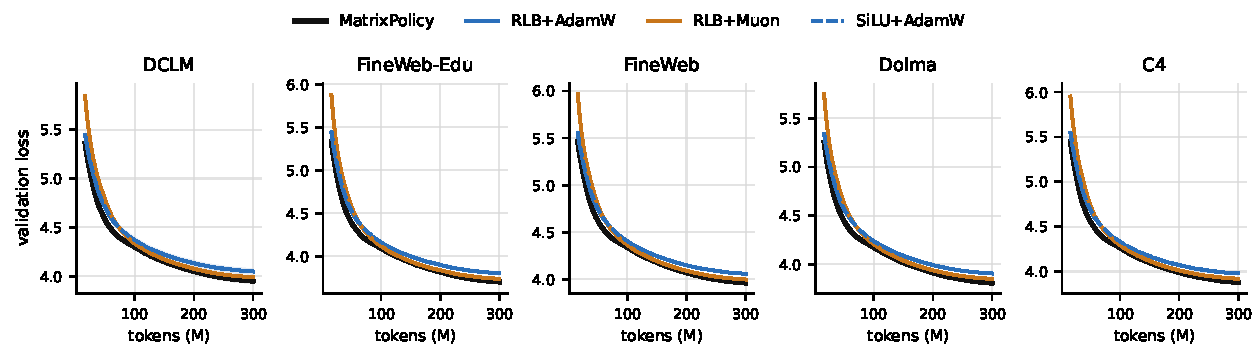
\includegraphics[width=0.99\linewidth]{figures/e2_validation_all_datasets.pdf}
\caption{E2 validation-loss trajectories on all five datasets.  Lines are means
over three seeds and bands are one sample standard deviation, plotted against
training tokens.  MatrixPolicy reaches the low-loss region earlier while retaining
an endpoint advantage after the full 300M-token budget.}
\label{fig:e2-trajectories}
\end{figure}

\subsection{Target Arrival and Training Time}
A fixed endpoint after a long budget does not answer how much training was needed
to reach a useful loss.  We therefore report first arrival at representative
validation-loss targets, measured at the native 50-step evaluation cadence.  For
each dataset we use targets reached by all three shared seeds for the comparator
view.  Figure~\ref{fig:target-time} plots saved tokens on the horizontal axis and
saved wall-clock minutes on the vertical axis, using measured per-method
throughput from completed JSONL summaries rather than Slurm queue time.  In E2,
MatrixPolicy saves 9.8--37.7M tokens against the fastest reachable
non-MatrixPolicy comparator and 51.9--69.9M tokens against SiLU+AdamW; these
readouts also give positive estimated time savings on every dataset.

\begin{figure}[H]
\centering
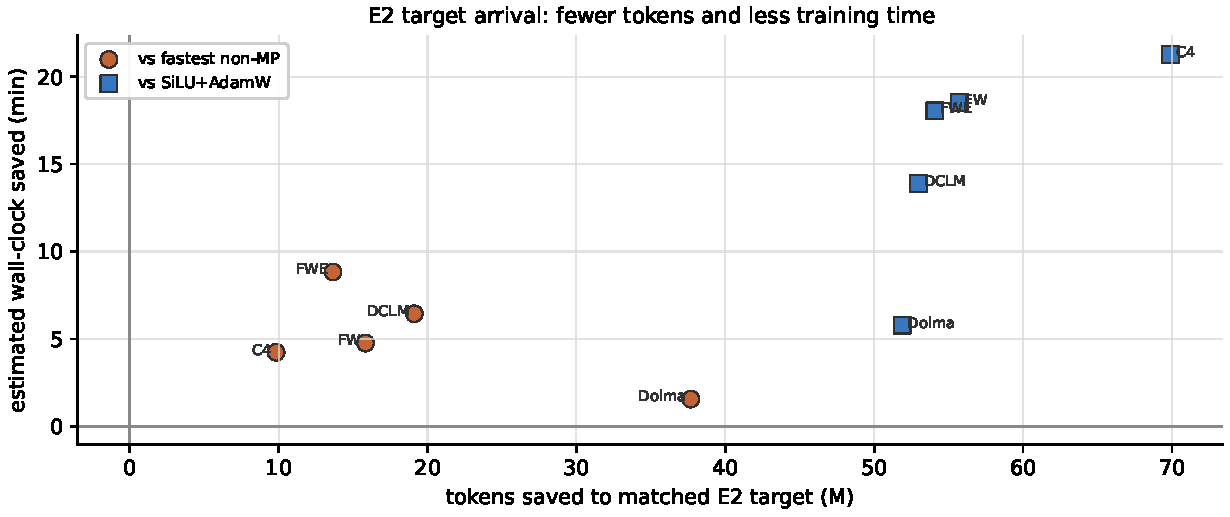
\includegraphics[width=0.86\linewidth]{figures/token_time_target_savings.pdf}
\caption{E2 token and estimated wall-clock savings at representative target
validation losses.  Each point is one dataset/comparator view.  Positive
horizontal and vertical coordinates mean MatrixPolicy reaches the same target
with fewer tokens and less estimated training time.}
\label{fig:target-time}
\end{figure}

\subsection{Endpoint Validation Loss}
Final validation loss still matters: a faster optimizer is not useful if it only
arrives early and then loses at the full budget.  Table~\ref{tab:final-loss}
therefore reports endpoint validation loss against the strongest aggregate
non-MatrixPolicy comparator in each dataset and regime.  MatrixPolicy is lower in
all ten fixed-budget comparisons.  The E2 gaps are smaller than the E1 gaps, as
expected in the longer saturation regime, but they remain positive after the full
300M-token budget.

\begin{table}[H]
\centering
\caption{Final validation loss under the fixed model protocol.  Values are mean
$\pm$ sample standard deviation over three seeds; lower is better.  MP denotes
MatrixPolicy.}
\label{tab:final-loss}
\scriptsize
\setlength{\tabcolsep}{2.5pt}
\resizebox{\linewidth}{!}{
\begin{tabular}{@{}lcccccc@{}}
\toprule
Dataset & E1 MP & E1 best non-MP & E1 gap & E2 MP & E2 best non-MP & E2 gap \\
\midrule
DCLM & $4.2538{\pm}0.0063$ & RLB+Lion $4.2946{\pm}0.0083$ & 0.0408 & $3.9518{\pm}0.0282$ & RLB+Lion $3.9887{\pm}0.0295$ & 0.0369 \\
FineWeb-Edu & $4.0873{\pm}0.0102$ & RLB+Lion $4.1361{\pm}0.0083$ & 0.0488 & $3.7015{\pm}0.0212$ & RLB+Muon $3.7373{\pm}0.0187$ & 0.0358 \\
FineWeb & $4.3162{\pm}0.0125$ & RLB+Lion $4.3626{\pm}0.0112$ & 0.0464 & $3.9623{\pm}0.0081$ & RLB+Lion $3.9960{\pm}0.0105$ & 0.0337 \\
Dolma-sample & $4.3253{\pm}0.0053$ & RLB+Lion $4.3622{\pm}0.0066$ & 0.0369 & $3.8062{\pm}0.0073$ & RLB+Lion $3.8412{\pm}0.0085$ & 0.0351 \\
C4 & $4.2837{\pm}0.0197$ & RLB+Lion $4.3271{\pm}0.0160$ & 0.0434 & $3.8777{\pm}0.0144$ & RLB+Lion $3.9132{\pm}0.0139$ & 0.0355 \\
\bottomrule
\end{tabular}
}
\end{table}

\subsection{Scale and Ablation Evidence}
The current evidence supports the fixed 12-layer, width-768 setting above.  The
next empirical layer is component attribution and scale transfer: direct ablations
of the MatrixPolicy group redistribution, transient matrix-direction branch, and
pair-balancing operation, followed by larger-model runs under the same
token-to-target and endpoint-loss readouts.  The present claims use only the
reported fixed-scale evidence.

\section{Related Work}
\label{sec:related}

Transformer nonlinear sublayers are often identified by their scalar response,
from GELU and Swish/SiLU to gated variants such as GLU and SwiGLU
\citep{hendrycks2016gelu,ramachandran2017swish,shazeer2020glu}.  RLB follows the
same architectural location but changes the interface exposed to optimization:
instead of replacing only a fixed scalar curve, it exposes grouped coordinates,
trainable rational responses, and the adjacent matrix roles used by MatrixPolicy.

Rational activations are motivated by the ability of low-degree rational
functions to represent sharp transitions, saturation, and curved response shapes
with few parameters.  Recent approximation-theoretic work argues that trainable
low-degree rational activations can have expressivity advantages over common
fixed activations \citep{tang2026rationalexpressivity}.  We use that result as
motivation for the activation family, not as a proof of MatrixPolicy.  The
empirical comparison separates the global-rational RLB sublayer from the
role-aware optimizer by including RLB controls with AdamW, Muon, Lion, SOAP,
CAME, and ScheduleFree-style optimizers.

Adam and AdamW remain standard Transformer pretraining optimizers
\citep{kingma2015iclr-adam,loshchilov2019decoupled}.  Other work changes the
first-order rule while keeping a generic tensor interface, including Lion and
cautious optimizers \citep{chen2023lion,liang2026cautious}, or uses matrix
structure and low-rank information, including Muon, Sophia, GaLore, SOAP, and
Adam-mini \citep{liu2025muon,liu2024sophia,zhao2024galore,vyas2025soap,zhang2025adammini}.
CAME and schedule-free training modify optimizer state or schedules
\citep{luo2023came,defazio2024road}.  MatrixPolicy is closest in spirit to
matrix-aware optimization, but it applies role-specific rules only to the input
and output matrices of RLB; all other Transformer parameters stay on AdamW.
Broader optimizer coverage is available in recent surveys \citep{wen2026fantastic}.

\section{Conclusion}
\label{sec:conclusion}

RLB turns the nonlinear Transformer sublayer into an optimizer-visible interface:
it exposes grouped normalized coordinates, trainable global rational responses,
and a positive matrix-pair structure.  MatrixPolicy uses that interface to update
the RLB input and output matrices with role-aware statistics while leaving the
rest of the model on AdamW.  The fixed-scale language-model experiments show a
consistent pattern: MatrixPolicy moves through useful E2 validation-loss targets
with fewer tokens and less estimated training time, and it preserves lower
endpoint validation loss after the full budget.  This supports the optimizer as a
mechanistic part of the result rather than an incidental wrapper around the
rational activation family.

\bibliography{references}
\bibliographystyle{iclr2026_conference}

\appendix

\section{Experimental Protocol and Supporting Evidence}
\label{app:experiment-protocol}

All runs use a 12-layer causal Transformer with width 768, 12 attention heads,
sequence length 256, RLB latent width 3072, and 32768 global tokens per optimizer
step.  E1 consists of 3050 optimizer steps and E2 consists of 9150 optimizer
steps.  Each method/dataset pair is run with seeds 1337, 2027, and 3407.  The
reported token-to-target readouts use evaluation events every 50 steps, so token
arrival is quantized in increments of 1.64M tokens.

The global-rational RLB rows use the no-local-atom activation: the active
nonlinearity is only the group-global P5/Q4 response in
\eqref{eq:global-rational-p}--\eqref{eq:global-rational-q}.  MatrixPolicy is
applied only to the RLB input and output matrices.  Rational coefficients,
attention weights, embeddings, normalization parameters, and all remaining
parameters use AdamW.  Non-MatrixPolicy controls keep the same model, token
budget, and dataset protocol while changing the optimizer and/or using the SiLU
baseline activation.

\begin{figure}[H]
\centering
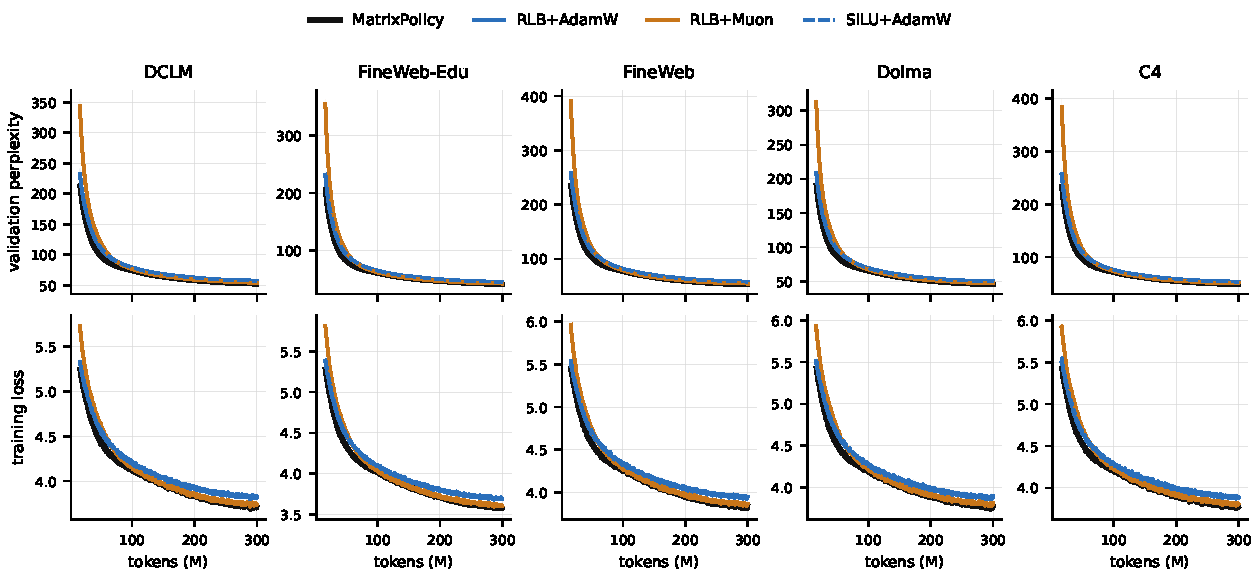
\includegraphics[width=0.99\linewidth]{figures/e2_auxiliary_dynamics.pdf}
\caption{E2 validation-perplexity and training-loss trajectories for the same
main comparator set as Figure~\ref{fig:e2-trajectories}.}
\label{app:auxiliary-curves}
\end{figure}

\begin{figure}[H]
\centering
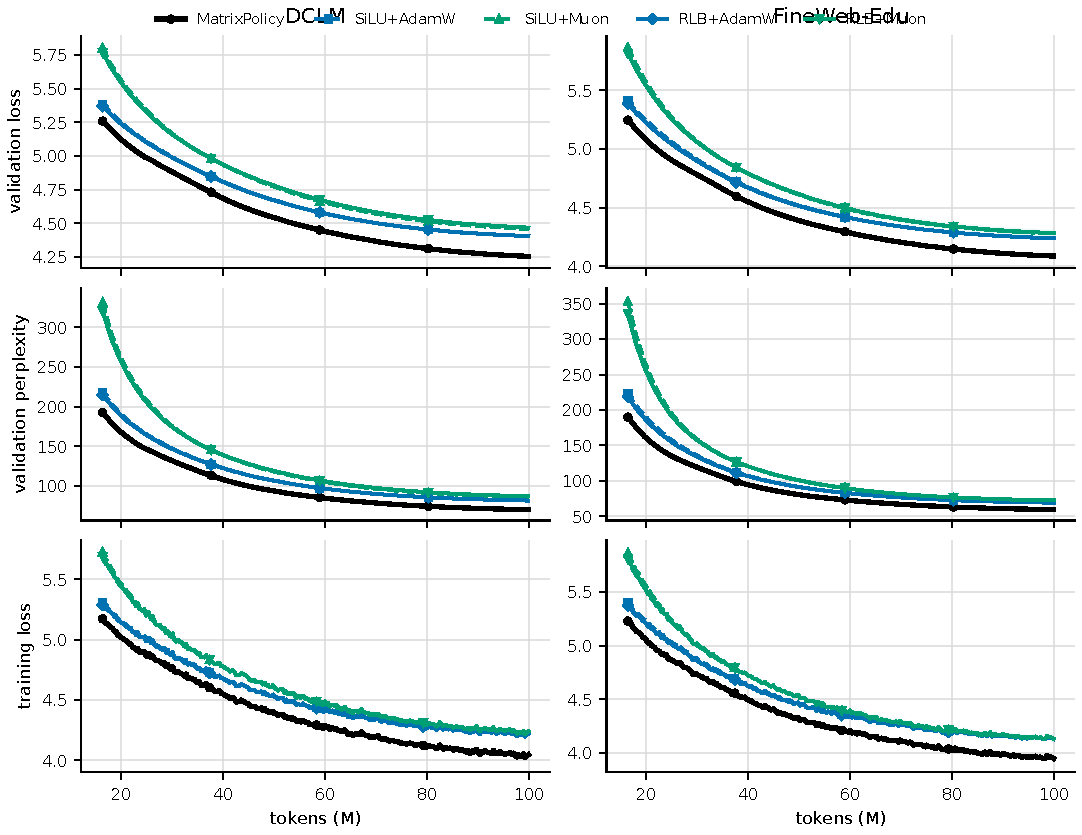
\includegraphics[width=0.92\linewidth]{figures/e1_multimetric_examples.pdf}
\caption{Representative E1 dynamics on DCLM and FineWeb-Edu.  E1 emphasizes the
earlier-budget separation; E2 in the main text emphasizes whether the advantage
survives after longer training.}
\label{app:e1-curves}
\end{figure}

\begin{table}[H]
\centering
\caption{Endpoint validation-loss gaps relative to MatrixPolicy across the five
datasets.  Positive gaps mean MatrixPolicy has lower final validation loss.}
\label{app:multi-comparator}
\small
\setlength{\tabcolsep}{4pt}
\begin{tabular}{@{}lcccc@{}}
\toprule
Comparator & E1 mean & E1 minimum & E2 mean & E2 minimum \\
\midrule
RLB+Lion & 0.043 & 0.037 & 0.036 & 0.034 \\
SiLU+Lion & 0.065 & 0.062 & 0.042 & 0.039 \\
RLB+Muon & 0.205 & 0.193 & 0.039 & 0.036 \\
SiLU+Muon & 0.203 & 0.191 & 0.047 & 0.044 \\
RLB+AdamW & 0.156 & 0.151 & 0.099 & 0.098 \\
SiLU+AdamW & 0.157 & 0.150 & 0.100 & 0.098 \\
RLB+SOAP & 0.220 & 0.162 & 0.125 & 0.109 \\
SiLU+SOAP & 0.171 & 0.162 & 0.153 & 0.145 \\
RLB+ScheduleFree & 0.687 & 0.633 & 0.422 & 0.406 \\
SiLU+ScheduleFree & 0.706 & 0.649 & 0.430 & 0.409 \\
RLB+CAME & 0.812 & 0.760 & 0.498 & 0.460 \\
SiLU+CAME & 0.817 & 0.757 & 0.441 & 0.416 \\
\bottomrule
\end{tabular}
\end{table}

\section{RLB Calculus and Matrix-Role Structure}
\label{app:rlb-calculus}

\subsection{Real-pole-free group-global response}
\label{app:rational-derivatives}

For one layer and group, write
\begin{align}
    P(u)=\sum_{i=0}^{5}a_i u^i,
    \qquad
    Q(u)=1+\sum_{j=1}^{4}|b_j|\phi_j(u),
    \qquad
    \phi(u)=(|u|,u^2,|u|^3,u^4).
\end{align}
Since $\phi_j(u)\ge 0$ for all real $u$, $Q(u)\ge 1$ and $R(u)=P(u)/Q(u)$ has
no real pole.  Away from the nondifferentiable point of the absolute-value term,
\begin{align}
    R'(u)
    =
    \frac{P'(u)Q(u)-P(u)Q'(u)}{Q(u)^2},
    \label{eq:appendix-r-prime}
\end{align}
where
\begin{align}
    P'(u)=\sum_{i=1}^{5} i a_i u^{i-1},
    \qquad
    Q'(u)=|b_1|\sign(u)+2|b_2|u+3|b_3|u|u|+4|b_4|u^3.
\end{align}
The implementation uses the autodiff convention $\sign(0)=0$ for derivative-gain
statistics.  The coefficient features are explicit:
\begin{align}
    \frac{\partial R(u)}{\partial a_i}=\frac{u^i}{Q(u)},
    \qquad
    \frac{\partial R(u)}{\partial b_j}
    =
    -\frac{P(u)}{Q(u)^2}\sign(b_j)\phi_j(u),
    \label{eq:appendix-coeff-features}
\end{align}
with the usual subgradient convention at zero.  These derivatives make output-factor
and derivative gains directly observable from the layer/group global curve,
without introducing local-atom parameters.

\subsection{Normalized-group Jacobian and gain summaries}
\label{app:rlb-jacobian}

For a group vector $z\in\mathbb{R}^{m}$, define
\begin{align}
    r(z)=\sqrt{m^{-1}\lVert z\rVert_2^2+\epsilon_{\rm rms}},
    \qquad
    u(z)=z/r(z),
    \qquad
    h(z)=r(z)R(u(z)),
\end{align}
where $R$ is applied coordinatewise.  The radius derivative is
\begin{align}
    \mathrm{d}r
    =
    \frac{z^\top \mathrm{d}z}{m r}
    =
    \frac{u^\top\mathrm{d}z}{m},
\end{align}
and the normalized-coordinate derivative is
\begin{align}
    \mathrm{d}u
    =
    \frac{1}{r}\left(I-\frac{uu^\top}{m}\right)\mathrm{d}z.
    \label{eq:appendix-du}
\end{align}
Therefore the group Jacobian is
\begin{align}
    J_h(z)
    :=
    \frac{\partial h}{\partial z}
    =
    R(u)\frac{u^\top}{m}
    +
    \diag(R'(u))\left(I-\frac{uu^\top}{m}\right).
    \label{eq:appendix-group-jacobian}
\end{align}
This decomposition motivates separate output-gain and derivative-gain summaries.
The vector $R(u)$ controls the curve-response factor inside the realized feature
$h=rR(u)$, while $R'(u)$ appears in the tangent component of the input Jacobian
seen by $A_l$.  The summaries $\hat o$ and $\hat d$ are not full feature-scale or
input-Jacobian measurements: the full feature also depends on $r$, and the full
input gradient also depends on the radial $R(u)u^\top/m$ term and on $B_{l,g}$.

\subsection{Positive matrix-pair rescaling with an RMS floor}
\label{app:positive-rescale}

Set $\epsilon_{\rm rms}=0$ and take $a>0$.  Then
\begin{align}
    r(az)=a r(z),
    \qquad
    u(az)=u(z),
    \qquad
    h(az)=a h(z).
\end{align}
Scaling $A_{l,g}$ by $a$ and the matching columns of $B_{l,g}$ by $a^{-1}$
therefore leaves the group contribution unchanged.  Applying this independently
to all groups gives \eqref{eq:positive-rescale}.

With $\epsilon_{\rm rms}>0$, define $r_\epsilon$ and $u_\epsilon$ by
\eqref{eq:rlb-normalization}.  For $\rho^2=m^{-1}\lVert z\rVert_2^2$,
\begin{align}
    u_\epsilon(az)
    =
    \kappa(a,z)u_\epsilon(z),
    \qquad
    \kappa(a,z)
    =
    \frac{a\sqrt{\rho^2+\epsilon_{\rm rms}}}
    {\sqrt{a^2\rho^2+\epsilon_{\rm rms}}}.
    \label{eq:appendix-kappa}
\end{align}
Let $L_R$ be a Lipschitz constant of the coordinatewise curve on the segment
between $u_\epsilon(z)$ and $\kappa(a,z)u_\epsilon(z)$.  After compensating the
output matrix by $a^{-1}$, the group-feature error obeys
\begin{align}
    \left\|a^{-1}h_\epsilon(az)-h_\epsilon(z)\right\|_2
    &\le
    \left|\frac{r_\epsilon(az)}{a}-r_\epsilon(z)\right|
    \left\|R(u_\epsilon(z))\right\|_2 \\
    &\quad+
    \frac{r_\epsilon(az)}{a}
    L_R |\kappa(a,z)-1|\left\|u_\epsilon(z)\right\|_2 .
    \label{eq:appendix-floor-bound}
\end{align}
Both terms vanish when $\epsilon_{\rm rms}=0$.  When
$\rho^2\gg \epsilon_{\rm rms}$ and the local response and slope are bounded on
the segment between $u_\epsilon(z)$ and $\kappa(a,z)u_\epsilon(z)$, the bound is
small; near the floor, the approximation can be poor.  This is the reason
MatrixPolicy uses clipped rescaling moves rather than treating matrix-pair
balancing as an exact function-preserving operation.


\section{MatrixPolicy Optimizer Step}
\label{app:matrixpolicy-step}

\begin{figure}[H]
\centering
\fbox{
\begin{minipage}{0.92\linewidth}
\textbf{MatrixPolicy update in one optimizer step.}
\begin{enumerate}
    \item Update moving averages of matrix-gradient scales and coefficient-gradient
    scales from current gradients.
    \item Read cached batch-estimated curve gains from the most recent RLB forward
    path.
    \item Step non-matrix parameters, including rational coefficients, with AdamW.
    \item Scale RLB matrix gradients with the centered group multipliers in
    \eqref{eq:group-center-clip}.
    \item Step RLB matrices with the AdamW matrix branch and any active Muon branch
    in \eqref{eq:matrix-branch-step}.
    \item Every five optimizer steps, apply the bounded positive matrix-pair
    rescaling in \eqref{eq:rescale-update}.
\end{enumerate}
\end{minipage}}
\caption{MatrixPolicy affects only the input and output matrices of RLB
sublayers.  All other parameters use the AdamW path.}
\label{app:matrixpolicy-step-figure}
\end{figure}
\section{MatrixPolicy Design Rationale}
\label{app:matrixpolicy-rationale}

\subsection{Role-specific gradients and gain selection}
\label{app:role-gradients}

For one training example, let $\bar y_l=\nabla_{y_l}\mathcal{L}$ be the upstream
gradient, and let $J_{l,g}=\partial h_{l,g}/\partial z_{l,g}$ be the group
Jacobian in \eqref{eq:appendix-group-jacobian}.  The two matrix gradients have
different forms:
\begin{align}
    \nabla_{B_{l,g}}\mathcal{L}
    =
    \bar y_l h_{l,g}^\top,
    \qquad
    \nabla_{A_{l,g}}\mathcal{L}
    =
    \left(J_{l,g}^\top B_{l,g}^\top\bar y_l\right)x_l^\top.
    \label{eq:appendix-matrix-gradients}
\end{align}
The output matrix sees the realized feature vector $h_{l,g}$ directly.  The
input matrix sees the upstream gradient filtered through $B_{l,g}$ and the RLB
group Jacobian.  This motivates using curve-response summaries for the output
role and derivative-gain summaries for the input role, while recognizing that
these summaries are proxies rather than full matrix preconditioners.

\subsection{Scale-normalized pressure and centered redistribution}
\label{app:pressure-redistribution}

The exact derivative along the homogeneous rescaling direction would be
\begin{align}
    \Delta_g
    =
    \left\langle\nabla_{A_{l,g}}\mathcal{L},A_{l,g}\right\rangle_F
    -
    \left\langle\nabla_{B_{l,g}}\mathcal{L},B_{l,g}\right\rangle_F.
    \label{eq:appendix-signed-pressure}
\end{align}
MatrixPolicy instead uses RMS relative gradient scales because they are stable
proxies for how strongly each matrix role is being moved.  For nonzero unfloored
$W$, if $W^+=W-\eta \mathcal{G}$ and $\eta$ is small, then
\begin{align}
    \log \rms(W^+)-\log\rms(W)
    =
    -\eta\frac{\langle \mathcal{G},W\rangle_F}{\lVert W\rVert_F^2}+O(\eta^2),
\end{align}
and Cauchy--Schwarz gives
\begin{align}
    \left|\frac{\langle \mathcal{G},W\rangle_F}{\lVert W\rVert_F^2}\right|
    \le
    \frac{\lVert \mathcal{G}\rVert_F}{\lVert W\rVert_F}
    =
    \frac{\rms(\mathcal{G})}{\rms(W)} .
    \label{eq:appendix-pressure-bound}
\end{align}
The implemented pressures are floored versions of this stable proxy, not natural
gradient terms.

Before clipping, the group policy is recentered by
\begin{align}
    \widehat c_{l,g,r}
    =
    \frac{c_{l,g,r}}{\geom_j c_{l,j,r}}.
\end{align}
Therefore
\begin{align}
    \frac{1}{G}\sum_{g=1}^{G}\log \widehat c_{l,g,r}
    =
    \frac{1}{G}\sum_{g=1}^{G}\log c_{l,g,r}
    -
    \log\left(\geom_j c_{l,j,r}\right)
    =0.
    \label{eq:appendix-centered-policy}
\end{align}
The centered policy redistributes group update scale while preserving the mean
log multiplier before clipping.  Clipping prevents noisy group statistics from
dominating a matrix update, at the cost of slightly perturbing the exact
zero-mean log property.

\subsection{Bounded matrix-pair balancing and transient direction updates}
\label{app:balancing-transient}

For the idealized nonzero-matrix calculation, let
\begin{align}
    \gamma_{l,g}=\log\rms(A_{l,g})-\log\rms(B_{l,g}).
\end{align}
The implementation uses the floored ratio in \eqref{eq:current-ratio}; near the
floor the exact contraction below is only an approximation.  On an active
positive-rescaling step,
$A_{l,g}\leftarrow e^{\ell_{l,g,t}}A_{l,g}$ and
$B_{l,g}\leftarrow e^{-\ell_{l,g,t}}B_{l,g}$, so the log ratio changes as
\begin{align}
    \gamma_{l,g}^{+}
    =
    \gamma_{l,g}+2\ell_{l,g,t}.
    \label{eq:appendix-gamma-update}
\end{align}
Ignoring clipping and writing $\lambda_{l,g,t}=s_{l,t}a^{\rm rs}_{l,g}$, the
update in \eqref{eq:rescale-log-step} gives
\begin{align}
    \gamma_{l,g}^{+}
    =
    (1-\lambda_{l,g,t})\gamma_{l,g}
    +
    \lambda_{l,g,t}\tau_{l,g}.
    \label{eq:appendix-rescale-contraction}
\end{align}
Thus, in the $\epsilon_{\rm rms}=0$ and unclipped idealization, each active
rescaling step moves the matrix representative toward the target ratio without
changing the represented homogeneous block map.  In the implemented setting this
operation runs every five optimizer steps, $\lambda_{l,g,t}$ is bounded by the
update schedule and activity factor, and the actual log move is clipped by
$0.030$.

The transient Muon branch uses the window
\begin{align}
    w(\xi_t)=\smooth(0.02,0.12,\xi_t)
    \left[1-\smooth(0.20,0.36,\xi_t)\right].
\end{align}
This confines the matrix-direction branch to the phase in which changes to
latent directions most directly affect the coordinates seen by the rational
curves.  The coefficient-gradient penalty $\psi_{l,t}$ further reduces the branch
when the rational coefficients are already moving strongly.  The design therefore
keeps the branch tied to the state of the RLB sublayer rather than applying a
persistent generic matrix rule throughout training.

\end{document}
